%#! platex UserGuideJa
\chapter{OpenFOAMのケース}
\label{chap:4}
\index{OpenFOAM!ケース}%
\index{ケース}%
本章では,OpenFOAMのケースのファイル構造について説明します.
通常,ユーザはケースに名前を割り当てます (例えばチュートリアルの
キャビティ流れのケースは単純に\OFcase{cavity}と名付けられています).
この名前は,すべてのケースファイルとサブディレクトリが
収納されているディレクトリの名前になります.
このケースディレクトリ自体はどこにでも置くことができますが,
\autoref{chap:2}の冒頭で述べたように,
\OFpath{\$HOME/OpenFOAM/\$\{USER\}-\OFversion}のように,
ユーザのプロジェクトのサブディレクトリ,
\index{run@\OFpath{run}!ディレクトリ}%
\index{ディレクトリ!run@\OFpath{run}}%
\OFpath{run}の中に置くことを推奨します.
この利点の一つは,
\index{FOAM RUN@\OFenv{FOAM\_RUN}!かんきょうへんすう@環境変数}%
\index{かんきょうへんすう@環境変数!FOAM RUN@\OFenv{FOAM\_RUN}}%
\OFenv{\$FOAM\_RUN}の環境変数がデフォルトで
\OFpath{\$HOME/OpenFOAM/\$\{USER\}-\OFversion/run}に設定されていることです.
コマンドラインでプリセットエイリアス,\OFpath{run}を実行することにより,
素早くこのディレクトリに移動することができます.
OpenFOAMをダウンロードする際に添付されているチュートリアルのケースは,
ケースのディレクトリ構造の有用な例を提供しています.
チュートリアルは\OFpath{\$FOAM\_TUTORIALS}のディレクトリに
置かれており,コマンドラインで\texttt{tut}エイリアスを
実行することにより素早くたどり着けます.
この章を読みながら,チュートリアルの例を参照してください.



\section{OpenFOAMのケースのファイル構造}
\label{sec:4.1}
アプリケーションを実行するために必要な最小限のファイルを含む,
OpenFOAMケースの基本的なディレクトリ構造を
\autoref{fig:4.1}に示し,以下で説明します.


\begin{figure}[ht]
 \begin{minipage}{.6\textwidth}
  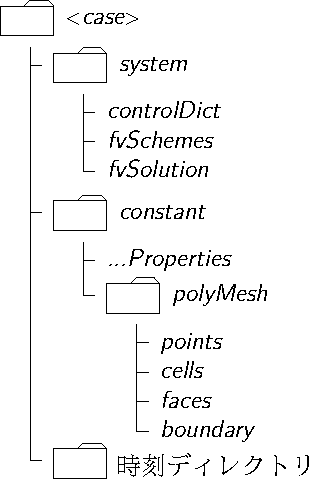
\includegraphics{fig-4-1}
  \hskip5pt
  \begin{minipage}[b]{7zw}
   \def\baselinestretch{1.2}\selectfont
   \autoref{sec:4.3}を参照\par
   \autoref{sec:4.4}を参照\par
   \autoref{sec:4.5}を参照\par
   \vskip28pt
   \autoref{chap:7}を参照\par
   \vskip4pt
   \autoref{ssec:5.1.2}を参照\par
   \vskip68pt
   \autoref{ssec:4.2.8}を参照\par
   \vskip-12pt\null
  \end{minipage}
 \end{minipage}
 \caption{ケースディレクトリの構造}
 \label{fig:4.1}
\end{figure}


\begin{description}
 \item[\OFpath{constant}ディレクトリ]
\index{constant@\OFpath{constant}!ディレクトリ}%
\index{ディレクトリ!constant@\OFpath{constant}}%
            そのケースのメッシュに関する全ての情報を含むサブディレクトリ
\index{polyMesh@\OFpath{polyMesh}!ディレクトリ}%
\index{ディレクトリ!polyMesh@\OFpath{polyMesh}}%
            \OFpath{polyMesh},
            および使おうとしているアプリケーションのための
            物性値を定めるファイル (例えば\OFdictionary{transportProperties}) が
            格納されています.
 \item[\OFpath{system}ディレクトリ]
\index{system@\OFpath{system}!ディレクトリ}%
\index{ディレクトリ!system@\OFpath{system}}%
            解析の手順に関連するパラメータ設定のための
            ディレクトリです.
            少なくとも以下の三つのファイルを含みます.
            パラメータが開始/終了時間や時間ステップ
            およびデータのアウトプットのためのパラメータの設定を行う
\index{controlDict@\OFdictionary{controlDict}!ディクショナリ}%
\index{ディクショナリ!controlDict@\OFdictionary{controlDict}}%
            \OFdictionary{controlDict},
            実行時に選択される解析に使われるスキームを
            記述している
\index{fvSchemes@\OFdictionary{fvSchemes}!ディクショナリ}%
\index{ディクショナリ!fvSchemes@\OFdictionary{fvSchemes}}%
            \OFdictionary{fvSchemes},
            そして実行のために方程式のソルバ,許容誤差およびその他の
            アルゴリズム制御を設定する
\index{fvSolution@\OFdictionary{fvSolution}!ディクショナリ}%
\index{ディクショナリ!fvSolution@\OFdictionary{fvSolution}}%
            \OFdictionary{fvSolution}です.
 \item[時刻ディレクトリ]
            特定のフィールドに関するデータの個別のファイルを含んでいます.
            データは,問題を定義するためにユーザが指定する
            初期値と境界条件,または書き込まれたOpenFOAMのファイルの
            結果が存在します.OpenFOAMのフィールドは,
            定常状態の問題のように厳密に解く必要のない場合であっても,
            常に初期化する必要があることに留意してください.
            各時刻ディレクトリの名称は,
            データが書き込まれた時点のシミュレーションが行われた
            時刻に基づいており,
            詳細については\autoref{sec:4.3}に記述されています.
            私達は通常時間$t = 0$でシミュレーションを始めて,
            初期条件は指定された名前のフォーマットに応じて
\index{0@\OFpath{0}!ディレクトリ}%
\index{ディレクトリ!0@\OFpath{0}}%
            \OFpath{0}または
\index{0.000000e+00@\OFpath{0.000000e+00}!ディレクトリ}%
\index{ディレクトリ!0.000000e+00@\OFpath{0.000000e+00}}%
            \OFpath{0.000000e+00}と名付けられたディレクトリの中に
            通常収納されるため,十分といえます.
            例えば,\OFcase{cavity}のチュートリアルで,
            速度場の$\bm{U}$と圧力場の$p$それぞれファイル
            \OFpath{O/U}と\OFpath{O/p}から初期化されます.
\end{description}



\section{基本的な入出力ファイルのフォーマット}
\label{sec:4.2}
\index{OpenFOAM!ファイルフォーマット}%
\index{ファイルフォーマット}%
OpenFOAMは,文字列,スカラ,ベクトル,テンソル,リスト,
およびフィールド等のデータ構造の範囲を読み込む必要があります.
入出力 (I/O) ファイルのフォーマットはユーザがOpenFOAMの
アプリケーションをできる限り容易に修正できるよう,
非常に柔軟に設計されています.
このI/Oは,ファイルの作成が非常に簡単で理解しやすい
単純なルールに従っているものであり,
ファイルのフォーマットが直観的に理解しづらいばかりか
どこにも公開されていないような,
多くのソフトウェアパッケージとは対照的です.
OpenFOAMのファイルフォーマットについては次節で説明します.


\subsection{一般的な構文規則}
\label{ssec:4.2.1}
フォーマットは以下のC++ソースコードの
いくつかの一般的な原理に従います.
\begin{itemize}
 \item ファイルは,列によって特定の意味が割り当てられることもなく,
       継続行を明示する必要もない,自由形式となっています.
 \item 行は特に意味をもちませんが,
\index{//@\verb+//+!OpenFOAMファイルこうぶん@OpenFOAMファイル構文}%
\index{OpenFOAMファイルこうぶん@OpenFOAMファイル構文!//@\verb+//+}%
       コメント・デリミタ \verb|//| があればOpenFOAMは行の最後までテキストを無視します.
 \item 複数行にわたるコメントは,\verb|/*| と \verb|*/| で囲みます.
\end{itemize}


\subsection{ディクショナリ}
\label{ssec:4.2.2}
OpenFOAMにおいてデータを指定する最も一般的な手段としては\emph{ディクショナリ}を使います.
ディクショナリには,\emph{キーワード}に応じてI/Oから読み出すことのできるデータ項目が含まれています.
キーワード・エントリは以下のような一般的な書式に従います.
\begin{OFverbatim}[file]
<keyword>  <dataEntry1> ... <dataEntryN>;
\end{OFverbatim}
ほとんどの入力項目は単一のデータ入力の書式になっています
\begin{OFverbatim}[file]
<keyword>  <dataEntry>;
\end{OFverbatim}
ほとんどのOpenFOAMのデータファイルはそれ自体1セットの
キーワード入力を含むディクショナリです.
ディクショナリは論理的なカテゴリにエントリを構成するための手段を提供しており,
階層的に指定できるので,
どんなディクショナリもそれ自体が一つ以上のディクショナリエントリを含んでいます.
ディクショナリの書式は,以下のようにディクショナリ名を指定し,
その後に波括弧 \verb|{ }| で囲まれたキーワード・エントリが続きます.
\begin{OFverbatim}[file]
<dictionaryName>
{
    ... keyword entries ...
}
\end{OFverbatim}


\subsection{データファイルヘッダ}
\label{ssec:4.2.3}
OpenFOAMによって読み書きされるすべてのデータファイルは,
\autoref{tbl:4.1}に記載されており,
キーワード入力の標準セットを含む
\index{FoamFile@\OFkeyword{FoamFile}!キーワード}%
\index{キーワード!FoamFile@\OFkeyword{FoamFile}}%
\OFkeyword{FoamFile}と
名付けられたディクショナリから始まります.


\begin{table}[ht]
 %#! platex UserGuideJa
\begin{tabularx}{\textwidth}{lXX}
 キーワード & 説明 & 入力 \\
 \hline
\index{version@\string\OFkeyword{version}!キーワード}%
\index{キーワード!version@\string\OFkeyword{version}}%
 \OFkeyword{version} & 入出力形式のバージョン & 2.0 \\
\index{format@\string\OFkeyword{format}!キーワード}%
\index{キーワード!format@\string\OFkeyword{format}}%
 \OFkeyword{format} & データ形式 & \OFkeyword{ascii} / \OFkeyword{binary} \\
\index{location@\string\OFkeyword{location}!キーワード}%
\index{キーワード!location@\string\OFkeyword{location}}%
 \OFkeyword{location} & ``...''ファイルへのパス & (オプション) \\
\index{class@\string\OFkeyword{class}!キーワード}%
\index{キーワード!class@\string\OFkeyword{class}}%
 \OFkeyword{class} & 関連するデータファイルから構成されたOpenFOAMのクラス &
         一般的に\OFkeyword{dictionary}もしくは領域,\hfil\break
         例:\OFkeyword{volVectorField} \\
\index{object@\string\OFkeyword{object}!キーワード}%
\index{キーワード!object@\string\OFkeyword{object}}%
 \OFkeyword{object} & ファイル名 & 例:\OFpath{controlDict} \\
 \hline
\end{tabularx}

 \caption{データファイルのためのヘッダのキーワード入力}
 \label{tbl:4.1}
\end{table}


この表には各エントリの簡単な説明を載せています.
これは\OFkeyword{class}については多くの例外があるものの,
おそらくほとんどのエントリについては十分な内容でしょう.
\OFkeyword{class}エントリはファイル内のデータから構成される
OpenFOAMライブラリでのC++クラスの名前です.
おそらくユーザは,読み込まれるファイルを呼び出す基礎的なコードの知識や
OpenFOAMクラスの知識なしに,
\OFkeyword{class}の入力を正確に推測することはできません.
しかし,ほとんどのデータファイルは単純なキーワードエントリをもち
内部の\OFclass{dictionary}クラスの中に読み込まれます.
それゆえ,それらの場合では\OFkeyword{class}エントリは\OFkeyword{dictionary}となります.

以下の例はこれまで説明してきたエントリのタイプを使った
ケースへのデータ供給のキーワードの使い方を示しています.
\OFdictionary{fvSolution}ディクショナリファイルを分解すると,
\OFdictionary{solvers}と\OFdictionary{PISO}という二つのディクショナリが含まれています.
\OFdictionary{solvers}ディクショナリは
圧力方程式と速度方程式に対してそれぞれ計算用と収束用に複数のデータ入力があり,
それぞれ\OFkeyword{p}と\OFkeyword{U}のキーワードによって記述されます.
\OFdictionary{PISO}ディクショナリはアルゴリズムの制御パラメータを含みます.
\begin{OFverbatim}[file, linenum=17]

solvers
{
    p
    {
        solver           PCG;
        preconditioner   DIC;
        tolerance        1e-06;
        relTol           0;
    }

    U
    {
        solver           PBiCG;
        preconditioner   DILU;
        tolerance        1e-05;
        relTol           0;
    }
}

PISO
{
    nCorrectors     2;
    nNonOrthogonalCorrectors 0;
    pRefCell        0;
    pRefValue       0;
}


// ************************************************************************* //
\end{OFverbatim}


\subsection{リスト}
\label{ssec:4.2.4}
OpenFOAMアプリケーションはリストを含んでいます.
例えば,メッシュ記述のための頂点リストがあります.
リストは一般的にI/Oにあり独自のフォーマットをもっていて,
入力は丸括弧 \verb|( )| 内にされます.
また,丸括弧の前のフォーマットの選択もあります.
\begin{description}
 \item[simple]
            キーワードに続いてすぐに丸括弧がくる.
\begin{OFverbatim}[file]
    <listName>
    (
        ... entries ...
    );
\end{OFverbatim}
 \item[numbered]
            キーワードに続いてリスト内の要素数 \verb|<n>| がくる.
\begin{OFverbatim}[file]
    <listName>
    <n>
    (
        ... entries ...
    );
\end{OFverbatim}
 \item[token identifier]
            キーワードに続いてクラス名の識別子ラベル \verb|<Type>| がくる.
            \verb|<Type>| はリストに何が入っているかを記載したもので,
            例えばスカラ要素のリストであれば次のようになる.
\begin{OFverbatim}[file]
    <listName>
    List<scalar>
    <n>        // optional
    (
        ... entries ...
    );
\end{OFverbatim}
\end{description}
ここで留意すべきはリスト \verb|<scalar>| での \verb|<scalar>| は
一般名ではなく入力された実際の文字列です.
単純なフォーマットは,リストを書くときの便利な方法です.
その他のフォーマットはリストのサイズがデータを読み込む前に
メモリに割り当てられるのでコードがより早くデータを読み込めます.
それゆえ単純なフォーマットは読み込み時間が最小の短いリストに適しており,
その他のフォーマットは長いリストに適しています.


\subsection{スカラとベクトル,テンソル}
\label{ssec:4.2.5}
スカラは,データファイルでは一つの数字として記述されます.
\index{vector@\OFclass{vector}!クラス}%
\index{クラス!vector@\OFclass{vector}}%
\OFclass{vector}は,ランク$1$で3\nobreak 次元の\OFemph{VectorSpace}であり,
要素数はいつも$3$に決まっているので単純なリストフォーマットで使われます.
それゆえ,ベクトル$(1.0,\ 1.1,\ 1.2)$は次のように書かれます.
\begin{OFverbatim}[file]
(1.0 1.1 1.2)
\end{OFverbatim}
OpenFOAMでは,テンソルはランク$2$で3\nobreak 次元の\OFemph{VectorSpace}であり,
それゆえデータ入力はいつも九つの実数と決まっています.
それゆえ単位テンソルは以下のように書かれます.
\begin{OFverbatim}[file]
(
    1 0 0
    0 1 0
    0 0 1
)
\end{OFverbatim}
この例は入力が複数の行に上書きできるように
OpenFOAMがその行に戻るのを無視する方法を示しています.
一行に数字を羅列することと扱いは違いません.
\begin{OFverbatim}[file]
( 1 0 0 0 1 0 0 0 1 )
\end{OFverbatim}


\subsection{次元の単位}
\label{ssec:4.2.6}
\index{じげんのたんい@次元の単位}%
連続体力学では,物理量はある決められた単位で表現されます.
例えば,質量ならキログラム ($\unit*{kg}$),体積なら立法メートル ($\unit*{m^{3}}$),
圧力ならパスカル ($\unit*{kg\,m^{-1}\,s^{-2}}$)というように.
代数の演算は統一した
\index{たんい@単位!そくりょう@測量\jdash}%
測量単位を用いて実行されなければなりません.
特に,足し算,引き算,および等式は同じ次元の単位の物理的特性においてのみ
意味があります.無意味な操作を実行することへの安全装置として,
OpenFOAMはフィールドデータと物理的特性に次元を付けて,
どのようなテンソル操作についても次元を
\index{じげん@次元!OpenFOAMにおけるチェック}%
チェックして実行します.
\OFkeyword{dimensionSet}の入出力形式は角括弧内の七つのスカラ量です.
例えば,
\begin{OFverbatim}[file]
[0 2 -1 0 0 0 0]
\end{OFverbatim}

\autoref{tbl:4.2}に記載するように
各値は計測基準単位のそれぞれの物理量に対応しています.
表は
\index{たんい@単位!SI}%
\index{たんい@単位!Syst\`eme International}%
国際単位系 (SI) と
\index{たんい@単位!USCS}%
\index{たんい@単位!United States Customary System}%
\index{USCS!たんい@単位}%
the United States Customary System (USCS) の
\index{たんい@単位!きほん@基本\jdash}%
基本単位ですが
OpenFOAMはどの単位系も使えます.
要求されることは入力データが選択した単位に合っているということです.
特に重要なのは,OpenFOAMがいくつかの次元化された物理定数を必要とする
ということを知っておくことです.
例えば熱力学のモデル化したある計算のための一般気体定数$R$などがいい例です.
これらの次元定数は
OpenFOAMインストール (\OFpath{\$WM\_PROJECT\_DIR/etc/controlDict}) の
メイン\OFdictionary{controlDict}ファイルの
\OFpath{DimensionedConstant}サブディクショナリで指定されます.
デフォルトでは,これらの定数はSIで設定されます.
USCSもしくはその他の単位系を使用したい場合は,
選択した単位系に合わせてこれらの定数を変更してください.


\begin{table}[t]
 %#! platex UserGuideJa
\begin{tabular}{clll}
\index{SIたんい@SI単位}%
 No. & 物理量 & SI単位 & USCS単位 \\
 \hline
 1 & 質量 & キログラム ($\unit*{kg}$) & 質量ポンド ($\unit*{lbm}$) \\
 2 & 長さ & メートル ($\unit*{m}$) & フィート ($\unit*{ft}$) \\
 3 & 時間 & \multicolumn{2}{c}{秒 ($\unit*{s}$)} \\
 4 & 温度 & ケルビン ($\unit*{K}$) & ランキン温度 ($\unit*{\degR}$) \\
 5 & 物質量 & モル ($\unit*{mol}$)\footnotemark & ポンドモル ($\unit*{lbmol}$) \\
 6 & 電流 & \multicolumn{2}{c}{アンペア ($\unit*{A}$)} \\
 7 & 光度 & \multicolumn{2}{c}{カンデラ ($\unit*{cd}$)} \\
 \hline
\end{tabular}

 \caption{SIとUSCSの基本単位}
 \label{tbl:4.2}
\end{table}
\footnotetext{訳注:原文では$\unit*{kgmol}$とされているが,これは誤り.
SIにおける物質量の基本単位は$\unit*{mol}$である.}%


\subsection{次元付きの型}
\label{ssec:4.2.7}
物理量は一般に,それらの関連する次元によって特定されます.
これらの入力は,\break
\OFkeyword{dimensionedScalar}の
以下の例が示すフォーマットをもっています.
\begin{OFverbatim}[file]
nu             nu  [0 2 -1 0 0 0 0]  1;
\end{OFverbatim}
最初の\OFkeyword{nu}はキーワード,2番目の\OFkeyword{nu}はクラスのwordの名前で,
通常キーワードと同じものが選ばれる.
その次の入力は\OFemph{dimensionSet}で最終的な入力はスカラ値です.


\subsection{フィールド}
\label{ssec:4.2.8}
OpenFOAMの入出力データの多くはテンソル場,
例えば速度や圧力のデータにあり,
時刻ディレクトリから読み込み時刻ディレクトリに書き込まれます.
\autoref{tbl:4.3}で説明されるように,
キーワード入力を使って,OpenFOAMはフィールドデータを書きこみます.


\begin{table}[ht]
 %#! platex UserGuideJa
\begin{tabular}{lll}
 キーワード & 説明 & 例 \\
 \hline
 \tblstrut
\index{dimensions@\OFkeyword{dimensions}!キーワード}%
\index{キーワード!dimensions@\OFkeyword{dimensions}}%
 \OFkeyword{dimensions} & 領域の次元 & \texttt{[1 1 -2 0 0 0 0]} \\
\index{internalField@\OFkeyword{internalField}!キーワード}%
\index{キーワード!internalField@\OFkeyword{internalField}}%
 \OFkeyword{internalField} & 内部領域の値 & \texttt{uniform (1 0 0)} \\
\index{boundaryField@\OFkeyword{boundaryField}!キーワード}%
\index{キーワード!boundaryField@\OFkeyword{boundaryField}}%
 \OFkeyword{boundaryField} & 境界領域 & \autoref{ssec:4.2.8}のファイル参照 \\
 \hline
\end{tabular}

 \caption{フィールドディクショナリで使われる主なキーワード}
 \label{tbl:4.3}
\end{table}


データは\OFkeyword{dimensions}エントリから始まります.
その後に続くのは,以下のいずれかの方法で記述される\OFkeyword{internalField}です.
\begin{description}
 \item[一様フィールド]
            ただひとつの値にそのフィールド内で全ての要素が対応していて,
            以下のような書式をとります.
\begin{OFverbatim}[file]
internalField uniform <entry>;
\end{OFverbatim}
 \item[非一様フィールド]
            各フィールドの要素は,固有の値を割り当てられ,
            リストの識別子トークンフォームにある
            以下の書式をとることが推奨されます.
\begin{OFverbatim}[file]
internalField nonuniform <List>;
\end{OFverbatim}
\end{description}
\OFpath{boundaryField}は\OFpath{polyMesh}ディレクトリ内の
\OFpath{boundary}ファイルにある境界パッチの
それぞれの名前に対応する名前の一連の入力を含んだディクショナリである.
各パッチの入力はそれ自体がキーワード入力のリストを含むディクショナリとなります.
必須エントリである\OFkeyword{type}には,
そのフィールドに指定すべきパッチ・フィールド条件を記述します.
残りの入力は選択されたパッチ・フィールド条件のタイプに対応し,
一般的にはパッチフェイスで初期条件を分類するフィールドデータを含みます.
OpenFOAMで使えるパッチ・フィールド条件の選択肢は,
その説明と指定しなければならないデータと併せて,
\autoref{tbl:5.3}と\autoref{tbl:5.4}に記載してあります.
速度\OFkeyword{U}のフィールドのディクショナリ入力の例を以下に示します.
\begin{OFverbatim}[file, linenum=17]
dimensions      [0 1 -1 0 0 0 0];

internalField   uniform (0 0 0);

boundaryField
{
    movingWall
    {
        type            fixedValue;
        value           uniform (1 0 0);
    }

    fixedWalls
    {
        type            fixedValue;
        value           uniform (0 0 0);
    }

    frontAndBack
    {
        type            empty;
    }
}

// ************************************************************************* //
\end{OFverbatim}


\subsection{ディレクティブとマクロ置換}
\label{ssec:4.2.9}
OpenFOAMのケースファイルを柔軟に設定するためのディレクティブや
代替マクロといったオプションのファイル構文があります.
ディレクティブはケースファイル内で \verb|#| から始まるコマンドとして記述されます.
代替マクロは \verb|$| から始まります.%$

OpenFOAMでは現在$4$種類のディレクティブが利用可能できます.
\begin{description}
 \item[\texttt{\char'043include "<fileName>"}]
            または \texttt{\char'043includeIfPresent "<fileName>"}
            \OFpath{<fileName>}という名前のファイルを読み込む
 \item[\texttt{\char'043inputMode}]
            二つのオプションがある.
            \OFkeyword{merge}は連続するディクショナリのキーワードのエントリを統合する.
            つまりある場所で指定されたキーワードのエントリを継承して
            以後の同一キーワードのエントリが指定される.
            \OFkeyword{overwrite}はディクショナリ全体を上書きする.
            通常は\OFkeyword{merge}を使う.
 \item[\texttt{\char'043remove <keywordEntry>}]
            インクルードされた全てのキーワードエントリを削除する.
            単語または正規表現で指定できる.
 \item[\texttt{\char'043codeStream}]
            続けてC++ソースコードを書くと,
            そのコードを即席でコンパイル・ロード・実行し,エントリを生成する.
\end{description}


\subsection{\texttt{\char'043include}および\hskip\xkanjiskip\texttt{\char'043inputMode}ディレクティブ}
\label{ssec:4.2.10@2.0.0}
一度使われた圧力の初期値を,内部フィールドと境界の初期値に設定する例を示します.
以下の記述を含む\OFpath{initialConditions}というファイルを作成していたとします.
\begin{OFverbatim}[file]
pressure 1e+05;
#inputMode merge
\end{OFverbatim}
この圧力をフィールド内部と境界に用いるために,
以下の代替マクロを圧力場のファイル\OFpath{p}に記述します.
\begin{OFverbatim}[file]
#include "initialConditions"
internalField uniform $pressure;
boundaryField
{
    patch1
    {
        type fixedValue;
        value $internalField;
    }
}
\end{OFverbatim}
あくまでもこれは,この機能がどのように働くかを示しただけの単純な例です.
しかしこの機能は,ケースデータをユーザのニーズに合わせて一般化する手段として,
より便利な使い方で多く用いることができます.
例えば同一のRAS乱流モデルの設定を用いるケースがいくつかある場合,
その設定を記述したファイルを一つ作成し,
各ケースの\OFpath{RSAProperties}ファイルに\texttt{include}によって
組み込めばよいのです.代替マクロは単独の値にとどまりません.
例えば,単独のマクロで境界条件のまとまりを事前に定義して,それをよびだすことができます.
この機能はほぼどこでも使えます.


\subsection{\texttt{\char'043codeStream}ディレクティブ}
\label{ssec:4.2.11@2.0.0}
\verb|#codeStream|ディレクティブはC++コードをコンパイル・実行して,
ディクショナリのエントリを生成します.
コードとコンパイル方法は以下のキーワードで指定します.
\begin{itemize}
 \item \texttt{code}: コードを指定します.
       これは\verb|OStream& os|および\verb|dictionary& dict|を引数とし,
       ユーザはコードの中でこれらの引数を使うことができます.
       例えば,当該ケースのディクショナリ(ファイル)から
       キーワード・エントリを取り出すことができます.
 \item \texttt{codeInclude}(オプション): OpenFOAMファイルを読み込むため,
       追加のC++ \verb|#include|文を指定できます.
 \item \texttt{codeOptions}(オプション): \OFpath{Make/options}の中の
       \verb|EXE_INC|に加えて,追加のコンパイル・フラグを指定できます.
 \item \texttt{codeLibs}(オプション): \OFpath{Make/options}の中の
       \verb|LIB_LIBS|に加えて,追加のコンパイル・フラグを指定できます.
\end{itemize}
コードは,ハッシュ・ブラケット記号,
すなわち\hskip\xkanjiskip\verb|#{...#}|\hskip\xkanjiskip で囲むことで,
通常の文字列と同じように複数行にわたって書くことができます.
この二つの記号の間のあらゆるものは,全ての改行・引用符などの予約語とともに,
一つの文字列となります.

以下に\hskip\xkanjiskip\verb|#codeStream|の例を示します.
このコードは\OFpath{controlDict}ファイル内に書かれており,
ディクショナリ・エントリを取り出し,出力間隔を決めるための簡単な計算を施しています.
\begin{OFverbatim}[file]
startTime       0;
endTime         100;
...
writeInterval   #codeStream
{
    code
    #{
        scalar start = readScalar(dict.lookup("startTime"));
        scalar end = readScalar(dict.lookup("endTime"));
        label nDumps = 5;
        os << ((end - start)/nDumps);
    #};
};
\end{OFverbatim}



\section{時間とデータの入出力制御}
\label{sec:4.3}
\index{じかんの@時間の!せいぎょ@制御}%
\index{せいぎょ@制御!じかんの@時間の\jdash}%
OpenFOAMのソルバは全て,
データベースをセットアップすることによって,動き始めます.
データベースは入出力を制御し,またデータの出力は通常実行中,
時間ごとに要求されるので,時間はデータベースにとって不可避の要素です.
\OFdictionary{controlDict}ディクショナリはデータベースの作成に不可欠な
入力パラメータを設定します.
\OFdictionary{controlDict}のキーワード入力項目は
\autoref{tbl:4.4}に記載されています.
時間制御方式と\OFkeyword{writeInterval}入力だけは完全に強制的で,
省略できる任意の項目には\autoref{tbl:4.4}で示された
デフォルト値のデータベースが用いられます.


\vskip\floatsep
\begingroup
 \small
% \begin{table}[ht]
 \LTXtable{\textwidth}{tbl/tbl-4-4}
 \addtocounter{table}{-1}%
 \tblcaption{controlDictディクショナリのキーワード項目}
 \label{tbl:4.4}
% \end{table}
\endgroup
\vskip\floatsep


以下に\OFdictionary{controlDict}ディクショナリの入力例を示します.
\begin{OFverbatim}[file, linenum=17]

application     icoFoam;

startFrom       startTime;

startTime       0;

stopAt          endTime;

endTime         0.5;

deltaT          0.005;

writeControl    timeStep;

writeInterval   20;

purgeWrite      0;

writeFormat     ascii;

writePrecision  6;

writeCompression off;

timeFormat      general;

timePrecision   6;

runTimeModifiable true;


// ************************************************************************* //
\end{OFverbatim}



\section{数値スキーム}
\label{sec:4.4}
\OFpath{system}ディレクトリにある
\index{fvSchemes@\OFdictionary{fvSchemes}!ディクショナリ}%
\index{ディクショナリ!fvSchemes@\OFdictionary{fvSchemes}}%
\OFdictionary{fvSchemes}ディクショナリは,
アプリケーションの実行時に現われる,
方程式における導関数等の項に対する数値スキームを設定します.
この節では,\OFdictionary{fvSchemes}ディクショナリにおいてどのように,
これらのスキームを指定するかを説明します.

\OFdictionary{fvSchemes}において数値スキームを割りあてなければならない典型的な項は,
例えば空間勾配といった導関数項や,
一つの点集合から他の集合へと値を補間する項等です.
OpenFOAMでは,ユーザに制限無くスキームを選択できるようにしたいと思っています.
例えば,線形補間は多くのケースで効率的ですが,
OpenFOAMでは,全ての補間項に対して幅広い補間スキームの中から
自由に選択ができるようになっています.

導関数の項は,このような選択の自由のさらなる好例となります.
ユーザは,まず離散化手法を選択することができますが,
ここではGaussによる有限体積積分を用いるのが一般的です.
Gauss積分は格子の界面における値を足していくことで実現されますが,
界面での値は格子中心での値から補間しなければなりません.
この補間スキームにおいてもユーザは自由に選ぶことができ,
特定の導関数項,特に対流項に用いる発散項には,
特別に設計されたいくつかのスキームが用意されています.
数値スキームを指定しなければならない項はいろいろありますが,
それらは\OFdictionary{fvSchemes}ディクショナリにおいて
\autoref{tbl:4.5}に示すカテゴリに分類されます.
\autoref{tbl:4.5}における各キーワードはサブディクショナリの名前ですが,
それらは各々特定のタイプの項を持っているわけです.
例えば,\OFkeyword{gradSchemes}には\OFkeyword{grad(p)}(と表現される)といった
全ての勾配項があります.
その他の例は,以下に示した
\index{fvSchemes@\OFdictionary{fvSchemes}!ディクショナリ}%
\index{ディクショナリ!fvSchemes@\OFdictionary{fvSchemes}}%
\OFdictionary{fvSchemes}ディクショナリの抜粋をご覧ください.


\begin{table}[ht]
 %#! platex UserGuideJa
\begin{tabular}{ll}
 キーワード & 数学的タームのカテゴリ \\
 \hline
\index{interpolationSchemes@\OFkeyword{interpolationSchemes}!キーワード}%
\index{キーワード!interpolationSchemes@\OFkeyword{interpolationSchemes}}%
 \OFkeyword{interpolationSchemes} & 2点間の値の補間 \\
\index{snGradSchemes@\OFkeyword{snGradSchemes}!キーワード}%
\index{キーワード!snGradSchemes@\OFkeyword{snGradSchemes}}%
 \OFkeyword{snGradSchemes} & 格子界面の法線方向勾配の各要素 \\
\index{gradSchemes@\OFkeyword{gradSchemes}!キーワード}%
\index{キーワード!gradSchemes@\OFkeyword{gradSchemes}}%
 \OFkeyword{gradSchemes} & 勾配$\nabla$ \\
\index{divSchemes@\OFkeyword{divSchemes}!キーワード}%
\index{キーワード!divSchemes@\OFkeyword{divSchemes}}%
 \OFkeyword{divSchemes} & 発散$\nabla \cdot {}$ \\
\index{laplacianSchemes@\OFkeyword{laplacianSchemes}!キーワード}%
\index{キーワード!laplacianSchemes@\OFkeyword{laplacianSchemes}}%
 \OFkeyword{laplacianSchemes} & Laplacian $\Laplacian$ \\
\index{timeScheme@\OFkeyword{timeScheme}!キーワード}%
\index{キーワード!timeScheme@\OFkeyword{timeScheme}}%
 \OFkeyword{timeScheme} & 1次と2次の時間導関数$\partial/\partial t$,$\partial^{2}/\partial^{2}t$ \\
\index{fluxRequired@\OFkeyword{fluxRequired}!キーワード}%
\index{キーワード!fluxRequired@\OFkeyword{fluxRequired}}%
 \OFkeyword{fluxRequired} & フラックスの生成が必要な物理量 \\
 \hline
\end{tabular}

 \caption{fvSchemesで使用する主なキーワード}
 \label{tbl:4.5}
\end{table}


\begin{OFverbatim}[file, linenum=17]

ddtSchemes
{
    default         Euler;
}

gradSchemes
{
    default         Gauss linear;
    grad(p)         Gauss linear;
}

divSchemes
{
    default         none;
    div(phi,U)      Gauss linear;
}

laplacianSchemes
{
    default         none;
    laplacian(nu,U) Gauss linear orthogonal;
    laplacian((1|A(U)),p) Gauss linear orthogonal;
}

interpolationSchemes
{
    default         linear;
    interpolate(HbyA) linear;
}

snGradSchemes
{
    default         orthogonal;
}

fluxRequired
{
    default         no;
    p;
}


// ************************************************************************* //
\end{OFverbatim}
この例を見ると\OFdictionary{fvSchemes}ディクショナリは
以下の要素から成り立っていることがわかります.
\begin{itemize}
 \item 六つの\OFsubdictionary{...Schemes}のサブディクショナリには,
       指定した各項に対するキーワードが書いてあり,
       \OFkeyword{default}のキーワードも指定できますが,
       その他にも,例えば$\nabla p$については\OFkeyword{grad(p)}というように,
       特定の項に対して名前を書くことで,
       それに対応するキーワードを指定することができます.
 \item \OFsubdictionary{fluxRequired}のサブディクショナリには,
       例えば\OFkeyword{p}のように,
       アプリケーションの中でフラックスが生成される場が書かれています.
\end{itemize}
もし,\OFkeyword{default}のスキームが
特定の\OFsubdictionary{...Schemes}のサブディクショナリで指定された場合には,
サブディクショナリが参照している全ての項にそのスキームが適用されます.
例えば,\OFsubdictionary{gradSchemes}において
\OFkeyword{default}が指定されている場合には,そのアプリケーションにおける,
$\nabla p$,$\nabla\bm{U}$といった全ての勾配項に対して,
その\OFkeyword{default}のスキームが適用されるわけです.
\OFkeyword{default}が指定されているときには,
そのサブディクショナリにおいて各項のスキームをいちいち指定する必要がなくなります.
この例では,\OFkeyword{grad(p)},\OFkeyword{grad(U)}の行がそれです.
しかしながら,特定の項の行が挿入された場合,
その項に対しては,指定されたスキームが\OFkeyword{default}より優先されます.

かわりに,ユーザは
\index{none@\OFkeyword{none}!キーワードエントリ}%
\index{キーワードエントリ!none@\OFkeyword{none}}%
\OFkeyword{none}エントリにより,
あえて\OFkeyword{default}スキームを使わないようにもできます.
この場合には,ユーザはそのサブディクショナリの中の全ての項を
個々に指定しなければなりません.
\OFkeyword{default}は上書きすることができるのですから,
\OFkeyword{default}に\OFkeyword{none}を設定することはやりすぎかもしれません.
しかしながら,\OFkeyword{none}を指定することは,
ユーザが全ての項を個別に指定しなければならないことから,
そのアプリケーションに実際にどの項が存在するかを認識するという点では有用です.

次の節では,\autoref{tbl:4.5}に示した
それぞれのカテゴリの項について,選択できるスキームを述べます.


\subsection{補間スキーム}
\label{ssec:4.4.1}
\OFsubdictionary{interpolationSchemes}サブディクショナリには,
通常,セル中心から界面中心へ値を内挿する項があります.
OpenFOAMでの内挿スキームの選択肢を
\autoref{tbl:4.6}に示しますが,
これは四つのカテゴリに分けられます.
一つのカテゴリは一般的なスキームが,そして他の三つのカテゴリは,
\autoref{ssec:4.4.5}で説明するように,
主に流体での対流(発散)項のGaussの離散化と一緒に使われるものです.
ユーザが\OFsubdictionary{interpolationSchemes}サブディクショナリにおいて,
対流特有のスキームを一般的なフィールドの内挿に適用することは,
「ほとんどない」のですが,有効な内挿スキームとして
\autoref{ssec:4.4.5}よりもむしろここで説明しておきます.
なお,
\index{UMIST@\OFkeyword{UMIST}!キーワードエントリ}%
\index{キーワードエントリ!UMIST@\OFkeyword{UMIST}}%
\OFkeyword{UMIST}のようなスキームもOpenFOAMでは
利用可能なことに注意すべきですが,
一般的に推奨されるスキームのみを\autoref{tbl:4.6}に示します.

普通のスキームは,単にキーワードとエントリのみを記すことで指定でき,
例えば\OFkeyword{linear}スキームを\OFkeyword{default}として指定するには
以下のようにします.
\begin{OFverbatim}[file]
default linear;
\end{OFverbatim}
対流特有のスキームは,流れの速度による流束に基づいて内挿を行います.
これらのスキームを指定する場合には,
内挿のベースとなる流束場の名前が必要ですが,
ほとんどのOpenFOAMのアプリケーションでは,
これは\OFkeyword{phi}となっており,この名前は,通常,
\OFkeyword{surfaceScalarField}の速度の流束に対応するものです.
このガイドの中では,対流特有のスキームの三つのカテゴリは,
general convection,normalised variable (NV),
そして,total variation diminishing (TVD) と記述されます.
\OFkeyword{blended}スキームを除いて,
general convectionとTVDスキームは,
そのスキーム名と流束場によって指定され,
例えば流束\OFkeyword{phi}に基づく\OFkeyword{upwind}スキームを
\OFkeyword{default}として指定するには以下のようにします.
\begin{OFverbatim}[file]
default upwind phi;
\end{OFverbatim}
いくつかのTVD/NVDスキームには,$0 \le \psi \le 1$の範囲の係数$\psi$が必要ですが,
$\psi = 1$はTVD条件に従うことに対応し,通常最も良い収束性を示すのに対し,
$\psi = 0$は最も良い精度を与えます.通常$\psi = 1$での実行がお勧めです.
流束\OFkeyword{phi}に基づく$\psi = 1.0$での\OFkeyword{limitedLinear}スキームを,
\OFkeyword{default}として指定するには以下のようにします.
\begin{OFverbatim}[file]
default limitedLinear 1.0 phi;
\end{OFverbatim}

\subsubsection{厳密に範囲が限定されるスカラ量に対するスキーム}
\label{sssec:4.4.1.1}
厳密に範囲が限定される必要のあるスカラ量のために,
いくつかの制限付きスキームという拡張版があります.
ユーザが指定した範囲に限定するためには,
スキームの名前には\OFkeyword{limited}という語が頭に付けられ,
下限と上限それぞれを続けて指定します.
例えば,\OFkeyword{vanLeer}スキームを$-2$と$3$の間で
厳密に制限するためには,次のように指定します.
\begin{OFverbatim}[file]
default limitedVanLeer -2.0 3.0;
\end{OFverbatim}
よく使われる$0$と$1$の間で限定されるスカラ場のために
特化された版もあります.
それらは,スキームの名前に\OFkeyword{01}を付けることで選択できます.
例えば,\OFkeyword{vanLeer}スキームを$0$と$1$の間で
厳密に限定するためには,以下のように指定します.
\begin{OFverbatim}[file]
default vanLeer01;
\end{OFverbatim}
厳密に範囲が限定する拡張版は,
\OFkeyword{limitedLinear},\OFkeyword{vanLeer},\OFkeyword{Gamma},
\OFkeyword{limitedCubic},\OFkeyword{MUSCL},\OFkeyword{SuperBee}の
スキームで利用することができます.

\subsubsection{ベクトル場に対するスキーム}
\label{sssec:4.4.1.2}
ベクトル場に対する制限付きスキームについては,
場の方向を考慮にいれて構成された改良版のリミッタがあります.
これらのスキームは,通常のスキームの名前に\OFkeyword{V}を
加えることで選択することができ,
\OFkeyword{limitedLinear}に対しては\OFkeyword{limitedLinearV}といった具合です.
これら\OFkeyword{V}版は\OFkeyword{limitedLinearV},\OFkeyword{vanLeerV},
\OFkeyword{GammaV},\OFkeyword{limitedCubicV},\OFkeyword{SFCDV}といったスキームで
利用することができます.


\begin{table}[ht]
 %#! platex UserGuideJa
\begin{tabular}{ll}
 \multicolumn{2}{l}{中心スキーム} \\
 \hline
 \tblstrut
\index{linear@\OFkeyword{linear}!キーワードエントリ}%
\index{キーワードエントリ!linear@\OFkeyword{linear}}%
 \OFkeyword{linear} & 線形補間(中心差分) \\
\index{cubicCorrection@\OFkeyword{cubicCorrection}!キーワードエントリ}%
\index{キーワードエントリ!cubicCorrection@\OFkeyword{cubicCorrection}}%
 \OFkeyword{cubicCorrection} & キュービックスキーム \\
\index{midPoint@\OFkeyword{midPoint}!キーワードエントリ}%
\index{キーワードエントリ!midPoint@\OFkeyword{midPoint}}%
 \OFkeyword{midPoint} & 均等重み付け線形補間 \\
 \\
 \multicolumn{2}{l}{風上対流スキーム} \\
 \hline
 \tblstrut
\index{upwind@\OFkeyword{upwind}!キーワードエントリ}%
\index{キーワードエントリ!upwind@\OFkeyword{upwind}}%
 \OFkeyword{upwind} & 風上差分 \\
\index{linearUpwind@\OFkeyword{linearUpwind}!キーワードエントリ}%
\index{キーワードエントリ!linearUpwind@\OFkeyword{linearUpwind}}%
 \OFkeyword{linearUpwind} & 線形風上差分 \\
\index{skewLinear@\OFkeyword{skewLinear}!キーワードエントリ}%
\index{キーワードエントリ!skewLinear@\OFkeyword{skewLinear}}%
 \OFkeyword{skewLinear} & ひずみ補正付き線形スキーム \\
\index{filteredLinear2@\OFkeyword{filteredLinear2}!キーワードエントリ}%
\index{キーワードエントリ!filteredLinear2@\OFkeyword{filteredLinear2}}%
 \OFkeyword{filteredLinear2} & 高周波の雑音のフィルタリングを伴う線形スキーム \\
 \\
 \multicolumn{2}{l}{TVDスキーム} \\
 \hline
 \tblstrut
\index{limitedLinear@\OFkeyword{limitedLinear}!キーワードエントリ}%
\index{キーワードエントリ!limitedLinear@\OFkeyword{limitedLinear}}%
 \OFkeyword{limitedLinear} & 有限線形差分 \\
\index{vanLeer@\OFkeyword{vanLeer}!キーワードエントリ}%
\index{キーワードエントリ!vanLeer@\OFkeyword{vanLeer}}%
 \OFkeyword{vanLeer} & van Leerリミッタ \\
\index{MUSCL@\OFkeyword{MUSCL}!キーワードエントリ}%
\index{キーワードエントリ!MUSCL@\OFkeyword{MUSCL}}%
 \OFkeyword{MUSCL} & MUSCLリミッタ \\
\index{limitedCubic@\OFkeyword{limitedCubic}!キーワードエントリ}%
\index{キーワードエントリ!limitedCubic@\OFkeyword{limitedCubic}}%
 \OFkeyword{limitedCubic} & キュービックリミッタ \\
 \\
 \multicolumn{2}{l}{NVDスキーム} \\
 \hline
 \tblstrut
\index{SFCD@\OFkeyword{SFCD}!キーワードエントリ}%
\index{キーワードエントリ!SFCD@\OFkeyword{SFCD}}%
 \OFkeyword{SFCD} & 自動フィルタ中心差分 \\
\index{Gamma@\OFkeyword{Gamma}!キーワードエントリ}%
\index{キーワードエントリ!Gamma@\OFkeyword{Gamma}}%
 \OFkeyword{Gamma} $\psi$ & ガンマ差分 \\
 \hline
\end{tabular}

 \caption{補間スキーム}
 \label{tbl:4.6}
\end{table}


\subsection{表面法線方向勾配スキーム}
\label{ssec:4.4.2}
\OFsubdictionary{snGradSchemes}サブディクショナリは,
表面法線方向勾配の項によるものです.
表面法線方向勾配は,格子の界面で計算されますが,
それは,界面が接続している二つの格子の中心における値の勾配の,
界面の法線方向の成分です.
表面法線方向勾配は,それ自体を使うためにも指定されますが,
Gauss積分を使ってLaplacianを評価する際にも必要となります.

利用可能なスキームを\autoref{tbl:4.7}に示しますが,
これらは単にキーワードとエントリを記述することで指定できます.
ただ,\OFkeyword{limited}は例外で,$0 \le \psi \le 1$の範囲の係数$\psi$を必要とします.
ここで,
\begin{align}
 \label{eq:4.1}
 \psi =
 \begin{cases}
  0 & \text{\OFkeyword{uncorrected}に対応}, \\
  0.333 & \text{非直交補正} \le 0.5 \times \text{直交部分}, \\
  0.5 & \text{非直交補正} \le \text{直交部分}, \\
  1.0 & \text{\OFkeyword{corrected}に対応}.
 \end{cases}
\end{align}
です.

よって,$\psi = 0.5$の\OFkeyword{limited}スキームを
\OFkeyword{default}として指定するには次のようにします.
\begin{OFverbatim}[file]
default limited 0.5;
\end{OFverbatim}


\begin{table}[ht]
 %#! platex UserGuideJa
\begin{tabular}{ll}
 スキーム & 説明 \\
 \hline
 \tblstrut
\index{corrected@\OFkeyword{corrected}!キーワードエントリ}%
\index{キーワードエントリ!corrected@\OFkeyword{corrected}}%
 \OFkeyword{corrected} & 陽的非直交補正 \\
\index{uncorrected@\OFkeyword{uncorrected}!キーワードエントリ}%
\index{キーワードエントリ!uncorrected@\OFkeyword{uncorrected}}%
 \OFkeyword{uncorrected} & 非直交補正なし \\
\index{limited@\OFkeyword{limited}!キーワードエントリ}%
\index{キーワードエントリ!limited@\OFkeyword{limited}}%
 \OFkeyword{limited} $\psi$ & 有限非直交補正 \\
\index{bounded@\OFkeyword{bounded}!キーワードエントリ}%
\index{キーワードエントリ!bounded@\OFkeyword{bounded}}%
 \OFkeyword{bounded} & ポジティブスカラの有界補正 \\
\index{fourth@\OFkeyword{fourth}!キーワードエントリ}%
\index{キーワードエントリ!fourth@\OFkeyword{fourth}}%
 \OFkeyword{fourth} & 4次 \\
 \hline
\end{tabular}

 \caption{表面法線方向勾配スキーム}
 \label{tbl:4.7}
\end{table}


\subsection{勾配スキーム}
\label{ssec:4.4.3}
\OFsubdictionary{gradSchemes}サブディクショナリには勾配項を記述します.
各項の離散化スキームは,\autoref{tbl:4.8}の中から
選択することができます.


\begin{table}[ht]
 %#! platex UserGuideJa
\begin{tabular}{ll}
 離散化スキーム & 説明 \\
 \hline
\index{Gauss@\OFkeyword{Gauss}!キーワードエントリ}%
\index{キーワードエントリ!Gauss@\OFkeyword{Gauss}}%
 \OFkeyword{Gauss} & 1次のガウス積分 \\
\index{leastSquares@\OFkeyword{leastSquares}!キーワードエントリ}%
\index{キーワードエントリ!leastSquares@\OFkeyword{leastSquares}}%
 \OFkeyword{leastSquares} & 2次の最小二乗法 \\
\index{fourth@\OFkeyword{fourth}!キーワードエントリ}%
\index{キーワードエントリ!fourth@\OFkeyword{fourth}}%
 \OFkeyword{fourth} & 4次の最小二乗法 \\
\index{limited@\OFkeyword{limited}!キーワードエントリ}%
\index{キーワードエントリ!limited@\OFkeyword{limited}}%
 \OFkeyword{limited} & 上記のスキームの制限バージョン \\
 \hline
\end{tabular}
 \caption{\OFsubdictionary{gradSchemes}において使用できる離散化スキーム}
 \label{tbl:4.8}
\end{table}


\OFkeyword{leastSquares}と\OFkeyword{fourth}の場合には,
離散化スキームの指定は次のように
そのスキーム名を指定するだけで十分です.
\begin{OFverbatim}[file]
grad(p) leastSqueares;
\end{OFverbatim}
\OFkeyword{Gauss}キーワードは,
Gauss積分による標準的な有限体積法の離散化を指定するもので,
これは,格子の中心から界面の中心への値の内挿を必要とします.
このため,\OFkeyword{Gauss}エントリでは,
\autoref{tbl:4.6}のような内挿スキームを続けて指定する必要があります.
一般的な内挿スキーム以外を選択することはほとんどなく,
ほとんどのケースでは次のように\OFkeyword{linear}スキームを選ぶのが効率的です.
\begin{OFverbatim}[file]
grad(p) Gauss linear;
\end{OFverbatim}
三つの基本的な勾配スキーム (\OFkeyword{Gauss},\OFkeyword{leastSquares},
\OFkeyword{fourth}) の範囲限定版は,
離散化スキームの前に
\OFkeyword{cellLimited} (または\OFkeyword{faceLimited}) を付けることで選択できます.
例えば,セルで制限されたGaussスキームは以下のようになります.
\begin{OFverbatim}[file]
grad(p) cellLimited Gauss linear 1;
\end{OFverbatim}


\subsection{Laplacianスキーム}
\label{ssec:4.4.4}
\OFsubdictionary{laplacianSchemes}サブディクショナリにはLaplacian項を記述します.
流体力学の中で見られる$\nabla \cdot (\rho\nabla\bm{U})$といった典型的なLaplacian項を
どのようにエントリに記述するかというと,
\OFkeyword{laplacian(nu, U)}といったword識別子で与えます.
離散化手法として選べるのは\OFkeyword{Gauss}スキームだけですが,
さらに拡散係数(この例では$\nu$)の内挿スキームや,
$\nabla\bm{U}$に対する表面法線方向勾配スキームの両方を選択する必要があります.
つまり,このエントリは以下のようになります.
\begin{OFverbatim}[file]
Gauss <interpolationScheme> <snGradScheme>
\end{OFverbatim}
内挿スキームは\autoref{tbl:4.6}から選択しますが,
通常は一般的なスキームから選択され,
ほとんどの場合\OFkeyword{linear}にします.
表面法線方向勾配スキームは\autoref{tbl:4.7}から選択し,
\autoref{tbl:4.9}に書かれているように
スキームの選択は数値的性質を決定します.
先の例でのLaplacian項の典型的なエントリは以下のようになります.
\begin{OFverbatim}[file]
laplacian(nu, U) Gauss linear corrected;
\end{OFverbatim}


\begin{table}[ht]
 %#! platex UserGuideJa
\begin{tabular}{ll}
 スキーム & 数値的性質 \\
 \hline
 \tblstrut
\index{corrected@\OFkeyword{corrected}!キーワードエントリ}%
\index{キーワードエントリ!corrected@\OFkeyword{corrected}}%
 \OFkeyword{corrected} & 無制限,2次,保存性 \\
\index{uncorrected@\OFkeyword{uncorrected}!キーワードエントリ}%
\index{キーワードエントリ!uncorrected@\OFkeyword{uncorrected}}%
 \OFkeyword{uncorrected} & 制限,1次,非保存性 \\
\index{limited@\OFkeyword{limited}!キーワードエントリ}%
\index{キーワードエントリ!limited@\OFkeyword{limited}}%
 \OFkeyword{limited} $\psi$ &
 \OFkeyword{corrected}と\OFkeyword{uncorrected}の混合 \\
\index{bounded@\OFkeyword{bounded}!キーワードエントリ}%
\index{キーワードエントリ!bounded@\OFkeyword{bounded}}%
 \OFkeyword{bounded} & 制限スカラの1次 \\
\index{fourth@\OFkeyword{fourth}!キーワードエントリ}%
\index{キーワードエントリ!fourth@\OFkeyword{fourth}}%
 \OFkeyword{fourth} & 無制限,4次,保存性 \\
 \hline
\end{tabular}
 \caption{\OFsubdictionary{laplacianSchemes}における表面法線方向スキームの性質}
 \label{tbl:4.9}
\end{table}


\subsection{発散スキーム}
\label{ssec:4.4.5}
\OFsubdictionary{divSchemes}サブディクショナリには発散項を記述します.
流体力学の中で見られる典型的な対流項$\nabla \cdot (\rho\bm{U}\bm{U})$はどうように記述するかというと,
OpenFOAMのアプリケーションでは通常\OFkeyword{div(phi, U)}という
識別子で与えます.ここで\OFkeyword{phi}はフラックス$\phi = \rho\bm{U}$です.

離散化手法として選べるのは\OFkeyword{Gauss}スキームだけですが,
さらに対象の場(この例では$\bm{U}$)の内挿スキームを選択する必要があります.
つまり,このエントリは以下のようになります.
\begin{OFverbatim}[file]
Gauss <interpolationScheme>
\end{OFverbatim}
内挿スキームは,一般的なものや対流特有のものも含め,
\autoref{tbl:4.6}の中から選択します.
この選択は,\autoref{tbl:4.10}に示すように,数値的性質を大きく決定づけます.
対流特有の内挿スキームを指定する場合でも,
流束は特定の項として既に値がわかっているものとし,
流束の内挿スキームは記述しません.
つまり,例えば\OFkeyword{div(phi, U)}の場合では,
流束は\OFkeyword{phi}として既知ですので,
さらにその内挿スキームを指定すると矛盾が生じるだけです.
よって,先の例での風上型内挿スキームの指定は次のようになります.
\begin{OFverbatim}[file]
div(phi, U) Gauss upwind;
\end{OFverbatim}


\begin{table}[ht]
 %#! platex UserGuideJa
\begin{tabular}{ll}
 スキーム & 数値的性質 \\
 \hline
\index{linear@\OFkeyword{linear}!キーワードエントリ}%
\index{キーワードエントリ!linear@\OFkeyword{linear}}%
 \OFkeyword{linear} & 2次,無制限 \\
\index{skewLinear@\OFkeyword{skewLinear}!キーワードエントリ}%
\index{キーワードエントリ!skewLinear@\OFkeyword{skewLinear}}%
 \OFkeyword{skewLinear} & 2次,(より) 無制限,ひずみ補正 \\
\index{cubicCorrected@\OFkeyword{cubicCorrected}!キーワードエントリ}%
\index{キーワードエントリ!cubicCorrected@\OFkeyword{cubicCorrected}}%
 \OFkeyword{cubicCorrected} & 4次,無制限 \\
\index{upwind@\OFkeyword{upwind}!キーワードエントリ}%
\index{キーワードエントリ!upwind@\OFkeyword{upwind}}%
 \OFkeyword{upwind} & 1次,制限 \\
\index{linearUpwind@\OFkeyword{linearUpwind}!キーワードエントリ}%
\index{キーワードエントリ!linearUpwind@\OFkeyword{linearUpwind}}%
 \OFkeyword{linearUpwind} & 1次/2次,制限 \\
\index{QUICK@\OFkeyword{QUICK}!キーワードエントリ}%
\index{キーワードエントリ!QUICK@\OFkeyword{QUICK}}%
 \OFkeyword{QUICK} & 1次/2次,制限 \\
 TVD schemes & 1次/2次,制限 \\
\index{SFCD@\OFkeyword{SFCD}!キーワードエントリ}%
\index{キーワードエントリ!SFCD@\OFkeyword{SFCD}}%
 \OFkeyword{SFCD} & 2次,制限 \\
 NVD schemes &  1次/2次,制限 \\
 \hline
\end{tabular}

 \caption{\OFsubdictionary{divSchemes}において使用される補間スキームの性質}
 \label{tbl:4.10}
\end{table}


\subsection{時間スキーム}
\label{ssec:4.4.6}
一次の時間微分項 ($\partial /\partial t$) は,
\OFsubdictionary{ddtSchemes}サブディクショナリで指定します.
各項に対する離散化スキームは\autoref{tbl:4.11}から選ぶことができます.

\OFkeyword{CrankNicholson}スキームでは,
\OFkeyword{Eular}スキームと混合させる割合を決める係数$\psi$を用います.
$\psi = 1$の場合には純粋な\OFkeyword{CrankNicholson},
$\psi = 0$の場合は純粋な\OFkeyword{Eular}に対応します.
純粋な\OFkeyword{CrankNicholson}では不安定なケースにおいては,
混合係数をいじることで計算を安定化させることができることがあります.


\begin{table}[ht]
 %#! platex UserGuideJa
\begin{tabular}{ll}
 スキーム & 説明 \\
 \hline
\index{Euler@\OFkeyword{Euler}!キーワードエントリ}%
\index{キーワードエントリ!Euler@\OFkeyword{Euler}}%
 \OFkeyword{Euler} & 1次,制限,陰的 \\
\index{localEuler@\OFkeyword{localEuler}!キーワードエントリ}%
\index{キーワードエントリ!localEuler@\OFkeyword{localEuler}}%
 \OFkeyword{localEuler} & 局所時間ステップ,1次,制限,陰的 \\
\index{CrankNicholson@\OFkeyword{CrankNicholson}!キーワードエントリ}%
\index{キーワードエントリ!CrankNicholson@\OFkeyword{CrankNicholson}}%
 \OFkeyword{CrankNicholson} $\psi$ & 2次,制限,陰的 \\
\index{backward@\OFkeyword{backward}!キーワードエントリ}%
\index{キーワードエントリ!backward@\OFkeyword{backward}}%
 \OFkeyword{backward} & 2次,陰的 \\
\index{steadyState@\OFkeyword{steadyState}!キーワードエントリ}%
\index{キーワードエントリ!steadyState@\OFkeyword{steadyState}}%
 \OFkeyword{steadyState} & 時間導関数について解かない \\
 \hline
\end{tabular}
 \caption{\OFsubdictionary{ddtSchemes}において使用可能な離散化スキーム}
 \label{tbl:4.11}
\end{table}


時間スキームを指定するときは,
非定常問題用のアプリケーションは定常状態で実行する必要はなく,
またその逆も同じであることに注意してください.
例えば,非定常の層流非圧縮流れのコードである
\OFtool{icoFoam}を実行するときに,
\OFkeyword{steadyState}(定常状態)を指定したら,
おそらく解は収束しないので,
定常の非圧縮流れのためには\OFtool{simpleFoam}を使うべきです.

2次時間微分項 ($\partial^{2}/\partial t^{2}$) は,
\OFsubdictionary{d2dt2Schemes}サブディクショナリの中で指定します.\break
\OFsubdictionary{d2dt2Schemes}としては,\OFkeyword{Euler}スキームのみが利用可能です.


\subsection{流束の算出}
\label{ssec:4.4.7}
\OFsubdictionary{fluxRequired}サブディクショナリには,
アプリケーションの中で流束を生成する場を書き出します.
例えば,多くの液体力学アプリケーションでは,
圧力の方程式を解くと流束が生成するので,
そのようなケースでは\OFsubdictionary{fluxRequired}サブディクショナリには
単に圧力のためのword識別子である\OFkeyword{p}を記載します.
\begin{OFverbatim}[file]
fluxRequired
{
    p;
}
\end{OFverbatim}



\section{解法とアルゴリズム制御}
\label{sec:4.5}
方程式のソルバ(求解機),公差,およびアルゴリズムは
\OFpath{system}ディレクトリの
\index{fvSolution@\OFdictionary{fvSolution}!ディクショナリ}%
\index{ディクショナリ!fvSolution@\OFdictionary{fvSolution}}%
\OFdictionary{fvSolution}ディクショナリから制御されます.
以下に示すのは,\OFtool{icoFoam}ソルバに必要な
\OFdictionary{fvSolution}ディクショナリからの入力例です.
\begin{OFverbatim}[file, linenum=17]

solvers
{
    p
    {
        solver           PCG;
        preconditioner   DIC;
        tolerance        1e-06;
        relTol           0;
    }

    U
    {
        solver           PBiCG;
        preconditioner   DILU;
        tolerance        1e-05;
        relTol           0;
    }
}

PISO
{
    nCorrectors     2;
    nNonOrthogonalCorrectors 0;
    pRefCell        0;
    pRefValue       0;
}


// ************************************************************************* //
\end{OFverbatim}%
\label{p:U-117}%
\OFdictionary{fvSolution}は実行されるソルバ特有のサブディクショナリを含んでいます.
しかしながら,標準のソルバに使われる\OFdictionary{fvSolution}の大部分は
標準的なサブディクショナリの小さなセットが占めています.
これらのサブディクショナリは本節の後半で説明する
\OFsubdictionary{solvers},\OFsubdictionary{relaxationFactors},\OFsubdictionary{PISO},
および\OFsubdictionary{SIMPLE}を含んでいます.


\subsection{線形ソルバ制御}
\label{ssec:4.5.1}
例題の最初のサブディクショナリであり,
すべてのソルバのアプリケーションに現れるサブディクショナリは
\index{solvers@\OFkeyword{solvers}!キーワード}%
\index{キーワード!solvers@\OFkeyword{solvers}}%
\OFkeyword{solvers}です.
ここには各離散化方程式に使用されるそれぞれの線形ソルバを指定します.
つまり強調すると,特定の問題を解くための
一連の方程式やアルゴリズムを意味するアプリケーションとしてのソルバとは対照的に,
線形ソルバという用語は一連の線形方程式の解くための数値演算方法のことを指します.
以下では,「線形ソルバ」という用語は「ソルバ」と省略されることが多くありますが,
その文脈によって曖昧さは避けられると思われます.

\OFsubdictionary{solvers}内の各エントリの構文には,
その方程式で解くべき変数を表す\OFclass{word}がキーワードとして用いられます.
例えば\OFtool{icoFoam}は,速度$\bm{U}$と圧力$p$の方程式を解くので,
\OFkeyword{U}および\OFkeyword{p}に対するエントリを書きます.
このキーワードの後には,ソルバのタイプと
このソルバが使うパラメータを含むディクショナリが続きます.
ソルバは,\autoref{tbl:4.12}に示すOpenFOAMでの選択肢から,
\index{solver@\OFkeyword{solver}!キーワード}%
\index{キーワード!solver@\OFkeyword{solver}}%
\OFkeyword{solver}キーワードで指定します.
\index{tolerance@\OFkeyword{tolerance}!キーワード}%
\index{キーワード!tolerance@\OFkeyword{tolerance}}%
\OFkeyword{tolerance},
\index{relTol@\OFkeyword{relTol}!キーワード}%
\index{キーワード!relTol@\OFkeyword{relTol}}%
\OFkeyword{relTol},
\index{preconditioner@\OFkeyword{preconditioner}!キーワード}%
\index{キーワード!preconditioner@\OFkeyword{preconditioner}}%
\OFkeyword{preconditioner}などのパラメータは次の節で説明します.


\begin{table}[ht]
 %#! platex UserGuideJa
\begin{tabular}{ll}
 ソルバ & キーワード \\
 \hline
 前処理付き(双)共役勾配 &
\index{PCG@\OFkeyword{PCG}!キーワードエントリ}%
\index{キーワードエントリ!PCG@\OFkeyword{PCG}}%
     \OFkeyword{PCG}/%
\index{PBiCG@\OFkeyword{PBiCG}!キーワードエントリ}%
\index{キーワードエントリ!PBiCG@\OFkeyword{PBiCG}}%
     \OFkeyword{PBiCG}\textsuperscript{\dag} \\
 スムーサを使ったソルバ &
\index{smoothSolver@\OFkeyword{smoothSolver}!キーワードエントリ}%
\index{キーワードエントリ!smoothSolver@\OFkeyword{smoothSolver}}%
     \OFkeyword{smoothSolver} \\
 汎用幾何学的代数マルチグリッド &
\index{GAMG@\OFkeyword{GAMG}!キーワードエントリ}%
\index{キーワードエントリ!GAMG@\OFkeyword{GAMG}}%
     \OFkeyword{GAMG} \\
 陽的な系のための対角ソルバ &
\index{diagonal@\OFkeyword{diagonal}!キーワードエントリ}%
\index{キーワードエントリ!diagonal@\OFkeyword{diagonal}}%
     \OFkeyword{diagonal} \\
 \hline
 {\footnotesize\dag\ \OFkeyword{PCG}は対称用,\OFkeyword{PBiCG}は非対称用}
\end{tabular}
 \caption{線形ソルバ}
 \label{tbl:4.12}
\end{table}


ソルバは対称行列と非対称行列を区別します.
行列の対称性は解かれている方程式の構造に依存し,
ユーザがこれを決定するこも可能ですが,
例えばOpenFOAMが不適当なソルバが選ばれているかどうかを
ユーザにアドバイスするためにエラーメッセージを出すので,
それは必須ではありません.
\begin{OFverbatim}[terminal]
--> FOAM FATAL IO ERROR : Unknown asymmetric matrix solver PCG
Valid asymmetric matrix solvers are :

(
PBiCG
smoothSolver
GAMG
)
\end{OFverbatim}

\subsubsection{解の許容範囲}
\label{sssec:4.5.1.1}
疎行列ソルバは反復計算,すなわち解の連続性により
方程式残差を減少させることに基づいています.
残差は表面上,解の誤差の尺度なので小さければ小さいほど,
より正確な解となります.
より正確にいえば,残差は,現在の解を方程式に代入して
左右両辺の差をとった大きさにより評価されたものです.
また,解析されている問題のスケールに依存しないように正規化されます.
特定のフィールドで方程式を解く前に,
初期の残差はそのフィールドの現在値に基づいて値を決めます.
それぞれのソルバの反復計算の後に,残差は再評価されます.
以下の条件のどちらかを満たせばソルバは停止します.
\begin{itemize}
 \item 残差が
\index{ソルバのきょようち@ソルバの許容値}%
\index{きょようち@許容値!ソルバの\jdash}%
       \emph{ソルバの許容値}以下に減少する,\OFkeyword{tolerance};
 \item 初期残差比率が
\index{ソルバのそうたいてきなきょようち@ソルバの相対的な許容値}%
\index{きょようち@許容値!ソルバのそうたいてきな@ソルバの相対的な\jdash}%
       ソルバの
\index{そうたいてきなきょようち@相対的な許容値}%
       \emph{相対的な許容値}以下に減少する,\OFkeyword{relTol};
 \item 反復回数が\emph{最大反復回数}を超える.\OFkeyword{maxIter};
\index{さいだい@最大!はんぷくかいすう@反復回数}%
\index{はんぷくかいすう@反復回数!さいだい@最大}%
\end{itemize}
ソルバの許容値は,その解が十分正確とみなせるくらい
残差が十分小さくなるようなレベルにしておくべきです.
ソルバの相対的な許容値は,初期値から最終的な解までの相対的な改善幅に制限をかけます.
非定常解析においては,各時刻ごとに解をソルバの許容値にしっかり収束させるために,
ソルバの相対的な許容値を$0$に設定するのが一般的です.
\OFkeyword{tolerance}および\OFkeyword{relTol}といった許容値は
全てのソルバに対してディクショナリで指定しなければなりませんが,
\OFkeyword{maxIter}はオプションです.


\subsubsection{前処理付き共役勾配ソルバ}
\label{sssec:4.5.1.2}
共役勾配ソルバには,さまざまな行列の前処理方法があり,
ソルバディクショナリの
\index{preconditioner@\OFkeyword{preconditioner}!キーワード}%
\index{キーワード!preconditioner@\OFkeyword{preconditioner}}%
\OFkeyword{precon\-ditioner}キーワードで指定します.
それらの前処理手法を\autoref{tbl:4.13}に記載します.


\begin{table}[ht]
 %#! platex UserGuideJa
\begin{tabular}{ll}
 前提条件 & キーワード \\
 \hline
 \tblstrut
 対角不完全Cholesky分解 (対称) &
\index{DIC@\OFkeyword{DIC}!キーワードエントリ}%
\index{キーワードエントリ!DIC@\OFkeyword{DIC}}%
     \OFkeyword{DIC} \\
 高速対角不完全Cholesky分解 (キャッシング付き\OFkeyword{DIC}) &
\index{FDIC@\OFkeyword{FDIC}!キーワードエントリ}%
\index{キーワードエントリ!FDIC@\OFkeyword{FDIC}}%
     \OFkeyword{FDIC} \\
 対角不完全LU (非対称) &
\index{DILU@\OFkeyword{DILU}!キーワードエントリ}%
\index{キーワードエントリ!DILU@\OFkeyword{DILU}}%
     \OFkeyword{DILU} \\
 対角 &
\index{diagonal@\OFkeyword{diagonal}!キーワードエントリ}%
\index{キーワードエントリ!diagonal@\OFkeyword{diagonal}}%
     \OFkeyword{diagonal} \\
 幾何学的代数マルチグリッド &
\index{GAMG@\OFkeyword{GAMG}!キーワードエントリ}%
\index{キーワードエントリ!GAMG@\OFkeyword{GAMG}}%
     \OFkeyword{GAMG} \\
 前処理なし &
\index{none@\OFkeyword{none}!キーワードエントリ}%
\index{キーワードエントリ!none@\OFkeyword{none}}%
     \OFkeyword{none} \\
 \hline
\end{tabular}
 \caption{前提条件オプション}
 \label{tbl:4.13}
\end{table}


\subsubsection{緩和法ソルバ}
\label{sssec:4.5.1.3}
緩和法を使うソルバにおいては,緩和法を指定する必要があります.
緩和法オプションを\autoref{tbl:4.14}に記載します.
一般に\OFkeyword{GaussSeidel}は最も信頼できるオプションですが,
行列がおかしい場合でも,\OFkeyword{DIC}であればより収束しやすくなります.
場合によっては\OFkeyword{GaussSeidel}による緩和も追加した,
いわゆる\OFkeyword{DICGaussSeidel}と呼ばれる方法がさらに有用です.


\begin{table}[ht]
 %#! platex UserGuideJa
\begin{tabular}{ll}
 緩和法 & キーワード \\
 \hline
 ガウス・ザイデル &
\index{GaussSeidel@\OFkeyword{GaussSeidel}!キーワードエントリ}%
\index{キーワードエントリ!GaussSeidel@\OFkeyword{GaussSeidel}}%
     \OFkeyword{GaussSeidel} \\
 対角不完全コレスキー分解(対称) &
\index{DIC@\OFkeyword{DIC}!キーワードエントリ}%
\index{キーワードエントリ!DIC@\OFkeyword{DIC}}%
     \OFkeyword{DIC} \\
 対角不完全コレスキー分解(対称)とガウス・ザイデル &
\index{DICGaussSeidel@\OFkeyword{DICGaussSeidel}!キーワードエントリ}%
\index{キーワードエントリ!DICGaussSeidel@\OFkeyword{DICGaussSeidel}}%
     \OFkeyword{DICGaussSeidel} \\
 \hline
\end{tabular}
 \caption{緩和法オプション}
 \label{tbl:4.14}
\end{table}


また,許容値パラメータに従って,
残差が再計算される前に\OFkeyword{nSweeps}というキーワードによって
スイープの数も定めなければなりません.


\subsubsection{代数幾何マルチグリッドソルバ}
\label{sssec:4.5.1.4}
\index{だいすうきかマルチグリッド@代数幾何マルチグリッド}%
\index{マルチグリッド!だいすうきか@代数幾何\jdash}%
代数幾何マルチグリッド (GAMG) の一般化された手法は
以下の原則に従います.セル数が少ないメッシュで素早く解を導きます.
そして,この解をより細かいメッシュに写します.
正確な解を出すのに細かいメッシュ上に初期の推測としてその値を使います.
最初により粗いメッシュを解くときの速度の増加が
メッシュ改良とフィールド・データに関するマッピングによる
負荷の増加より重いときに,GAMGは標準の方法より速くなります.
実際には,GAMGは指定されたメッシュから計算を始め,
徐々にメッシュを粗くもしくは細かくしていきます.
ユーザはセルの\OFkeyword{nCoarsestCells}の数に関して
最も粗いレベルにおける大体のメッシュサイズを指定するだけで構いません.
セルの統合は
\index{agglomerator@\OFkeyword{agglomerator}!キーワード}%
\index{キーワード!agglomerator@\OFkeyword{agglomerator}}%
\OFkeyword{agglomerator}キーワードによって指定された
アルゴリズムで実行されます.
今のところ,
\index{faceAreaPair@\OFkeyword{faceAreaPair}!キーワードエントリ}%
\index{キーワードエントリ!faceAreaPair@\OFkeyword{faceAreaPair}}%
\OFkeyword{faceAreaPair}法を薦めます.
\OFkeyword{MGridGen}の共有されたオブジェクト・ライブラリを指定する追加入力が必要な
\index{MGridGen@\OFkeyword{MGridGen}!キーワードエントリ}%
\index{キーワードエントリ!MGridGen@\OFkeyword{MGridGen}}%
\OFkeyword{MGridGen}オプションがあることに注意する必要があります.
\begin{OFverbatim}[file]
geometricGamgAgglomerationLibs ("libMGridGenGamgAgglomeration.so");
\end{OFverbatim}
OpenCFDの経験によれば,
\href{http://www-users.cs.umn.edu/~moulitsa/software.html}{MGridGen}メソッドよりも
\OFkeyword{faceAreaPair}メソッドの方が優れています.
すべての方法において,
\index{cacheAgglomeration@\OFkeyword{cacheAgglomeration}!キーワード}%
\index{キーワード!cacheAgglomeration@\OFkeyword{cacheAgglomeration}}%
\OFkeyword{cacheAgglomeration}スイッチによって
統合を任意にキャッシュできます.
緩和法は\autoref{sssec:4.5.1.3}で説明したように
\index{smoother@\OFkeyword{smoother}!キーワード}%
\index{キーワード!smoother@\OFkeyword{smoother}}%
\OFkeyword{smoother}によって指定されます.
その緩和法が各メッシュ密度レベルにおいて実行されるスイープ回数は
\index{nPreSweeps@\OFkeyword{nPreSweeps}!キーワード}%
\index{キーワード!nPreSweeps@\OFkeyword{nPreSweeps}}%
\OFkeyword{nPreSweeps}や
\index{nPostSweeps@\OFkeyword{nPostSweeps}!キーワード}%
\index{キーワード!nPostSweeps@\OFkeyword{nPostSweeps}}%
\OFkeyword{nPostSweeps},
\index{nFinestSweeps@\OFkeyword{nFinestSweeps}!キーワード}%
\index{キーワード!nFinestSweeps@\OFkeyword{nFinestSweeps}}%
\OFkeyword{nFinestSweeps}のキーワードによって指定されます.
\index{nPreSweepsh@\OFkeyword{nPreSweepsh}!キーワード}%
\index{キーワード!nPreSweepsh@\OFkeyword{nPreSweepsh}}%
\OFkeyword{nPreSweepsh}への入力はアルゴリズムがメッシュを粗くするときに使われ,
\index{nPostSweeps@\OFkeyword{nPostSweeps}!キーワード}%
\index{キーワード!nPostSweeps@\OFkeyword{nPostSweeps}}%
\OFkeyword{nPostSweeps}への入力はアルゴリズムがメッシュを細分割するときに使われ,
\index{nFinestSweeps@\OFkeyword{nFinestSweeps}!キーワード}%
\index{キーワード!nFinestSweeps@\OFkeyword{nFinestSweeps}}%
\OFkeyword{nFinestSweeps}は解が最も細かいレベルにあるときに使われます.

\index{mergeLevels@\OFkeyword{mergeLevels}!キーワード}%
\index{キーワード!mergeLevels@\OFkeyword{mergeLevels}}%
\OFkeyword{mergeLevels}キーワードは,
レベルを粗く,もしくは細かくするスピードを制御します.
多くの場合は1レベルずつ,すなわち\texttt{mergeLevels 1}のように設定するのが最適です.
場合によって,特に簡単なメッシュに関しては,
例えば\texttt{mergeLevels 2}のように一度に2レベル粗く
または細かくすることによって,解析を確実に早くできます.


\subsection{不足緩和解析}
\label{ssec:4.5.2}
OpenFOAMでよく使われる\OFdictionary{fvSolution}の2番目のサブディクショナリは
緩和して制御する\OFsubdictionary{relaxationFactors}で,
計算の安定性を改良するのに使用されるテクニックなのですが,
特に定常状態問題を解析する際に使われます.
緩和は,領域の解析の前に解のマトリックスとソースを変更するか,
または直接領域を変更することによって,
反復計算時の変数の変化を制限することで行われます.
緩和係数$\alpha$ ($0 < \alpha \le 1$) は緩和の量を指定し,
$0$から$\alpha = 1$まで変化し,強さは$\alpha \to 0$に従って増加します.
$\alpha = 0$は連続した反復計算で変数を全く変化させない場合の解であり,
極端なケースです.最適な$\alpha$の選択は
安定した計算を確実にすることができるくらい小さく,
また反復計算をスムーズに進められる程度大きくしなければなりません.
$\alpha$の値が$0.9$程度であれば安定性を確保できることがありますが,
著しく低い値,例えば$0.2$といった値は,
反復計算を遅くするためほとんど使われることはありません.
ユーザは,その場と係数に関連している\OFkeyword{word}を
最初に指定することによって,特定の場に対して緩和係数を指定できます.
以下に,非圧縮定常状態層流の
\OFtool{simpleFoam}のチュートリアルの例で使われている緩和係数を示します.
\begin{OFverbatim}[file, linenum=17]

solvers
{
    p
    {
        solver          PCG;
        preconditioner  DIC;
        tolerance       1e-06;
        relTol          0.01;
    }

    U
    {
        solver          PBiCG;
        preconditioner  DILU;
        tolerance       1e-05;
        relTol          0.1;
    }

    k
    {
        solver          PBiCG;
        preconditioner  DILU;
        tolerance       1e-05;
        relTol          0.1;
    }

    epsilon
    {
        solver          PBiCG;
        preconditioner  DILU;
        tolerance       1e-05;
        relTol          0.1;
    }

    R
    {
        solver          PBiCG;
        preconditioner  DILU;
        tolerance       1e-05;
        relTol          0.1;
    }

    nuTilda
    {
        solver          PBiCG;
        preconditioner  DILU;
        tolerance       1e-05;
        relTol          0.1;
    }
}

SIMPLE
{
    nNonOrthogonalCorrectors 0;

    residualControl
    {
        p               1e-2;
        U               1e-3;
        "(k|epsilon|omega)" 1e-3;
    }
}

relaxationFactors
{
    fields
    {
        p               0.3;
    }
    equations
    {
        U               0.7;
        k               0.7;
        epsilon         0.7;
        R               0.7;
        nuTilda         0.7;
    }
}


// ************************************************************************* //
\end{OFverbatim}


\subsection{PISOとSIMPLEアルゴリズム}
\label{ssec:4.5.3}
OpenFOAMのほとんどの流体力学ソルバアプリケーションは,
pressure-implicit split-operator (PISO) もしくは
semi-implicit method for pressure-linked equations
(SIMPLE) アルゴリズムを使用します.
これらのアルゴリズムは,速度と圧力の方程式を解くための反復法で,
PISOは非定常状態の問題に,SIMPLEは定常状態の問題に使います.

両アルゴリズムはいくつかの初期解を求め,
次に,それらを修正するという方法をとります.
SIMPLEは1段階の修正しかしませんが,PISOは1段階以上で,大概は4段階以下の修正をします.
したがって,\pageref{p:U-117}ページの入力例に示したように\OFkeyword{nCorrectors}キーワードで
\OFdictionary{PISO}ディクショナリの補正数を定めます.

非直交性メッシュからなる追加補正は標準のOpenFOAMソルバアプリケーションの
SIMPLEとPISOの両方で利用できます.
例えば面が直行座標系に並べられる6面体のセルのメッシュのように,
メッシュ内の各面において隣接するセルの中心間のベクトルに面が平行であるなら,
メッシュは直交しています.
非直交の補正数は\pageref{p:U-117}ページの入力例に示すように
\OFkeyword{nNonOrthogonalCorrectors}キーワードによって定めます.
例えば,直交メッシュを$0$として非直交性の度合いによって
最大で$20$まで増加するようにするなど
非直交の補正数は解くケースのメッシュに対応させます.

\subsubsection{圧力の参照}
\label{sssec:4.5.3.1}
非圧縮の閉鎖系では圧力は相対的で,
重要なのは絶対値ではなく範囲です.
この場合,ソルバはセル内の
\index{pRefValue@\OFkeyword{pRefValue}!キーワード}%
\index{キーワード!pRefValue@\OFkeyword{pRefValue}}%
\OFkeyword{pRefValue}の基準面を,
\OFkeyword{p}が圧力の変数解の名前の場合,
\index{pRefCell@\OFkeyword{pRefCell}!キーワード}%
\index{キーワード!pRefCell@\OFkeyword{pRefCell}}%
\OFkeyword{pRefCell}に設定します.
圧力が\OFkeyword{p\_rgh}であるところでは,
名前はそれぞれ
\index{p rghRefValue@\OFkeyword{p\_rghRefValue}!キーワード}%
\index{キーワード!p rghRefValue@\OFkeyword{p\_rghRefValue}}%
\OFkeyword{p\_rghRefValue}と
\index{p rghRefCell@\OFkeyword{p\_rghRefCell}!キーワード}%
\index{キーワード!p rghRefCell@\OFkeyword{p\_rghRefCell}}%
\OFkeyword{p\_rghRefCell}です.
これらの入力は,一般に\OFsubdictionary{PISO}/\OFsubdictionary{SIMPLE}サブディクショナリに格納されて,
ケースに応じてソルバがそれらを必要としたときに使われます.
もしこれを忘れるとソルバは実行されずに,エラーメッセージが出ます.


\subsection{その他のパラメタ}
\label{ssec:4.5.4}
標準のOpenFOAMソルバアプリケーションの多くの\OFdictionary{fvSolutions}ディクショナリには,
これまで本節で説明した以外の項目はありません.
しかし,一般に,\OFdictionary{fvSolution}ディクショナリはソルバ,アルゴリズム,
または実際の何かを制御するどんなパラメータをもっていてもおかしくありません.
どんなソルバでも,必要なパラメタを把握するために
ソースコードを見ることができます.
結局,何かパラメータやサブディクショナリがなければ,
ソルバが実行されるとき,
詳細なエラーメッセージが印字されて終了するでしょう.
そのとき,それに応じて不足のパラメータを加えてください.

